\scanpage{105}
% archive sheet number: 104
$\pi_2(X,\xi)$

a) Si $X$ simplement connexe
alors $M\unsure{\leadsto|\sim}H^2(X,M)$
avec $M$ \deleted{\unsure{faisceau de}}\inserted{groupe de} torsion \deleted{\unsure{entier}} fini
est exact à g., donc proreprésentable par
\[
H^2(X,M)=\operatorname{Hom\,cont}(\underline{\pi_2(X)},M)
\]

b) Dans le cas général, $\pi_2(X,\xi)=\pi_2(\widetilde{X(\xi)})$
\margin{\unsure{revêtemt|revêtt} universel \unsure{pointé|pointu} défini par $\xi$}

\figure{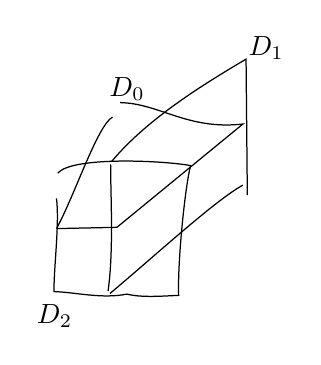
\begin{tikzpicture}[x=.80cm,y=.80cm,line width=.45pt]
\draw (0,1.48) .. controls (.05,1.1) and (-.04,.4) .. (-.04,0)
 .. controls (.30,-.01) and (.72,-.12) .. (1.12,-.04)
 .. controls (1.35,-.10) and (1.70,-.07) .. (1.94,-.06)
 .. controls (1.92,.46) and (2.04,1.66) .. (2.13,2)
 .. controls (1.70,2.08) and (.25,2.15) .. (.02,1.88);
\draw (.82,.01) .. controls (.91,.67) and (.86,1.5) .. (.86,2.02);
\draw (.88,2.07) .. controls (1.45,2.75) and (2.35,3.3) .. (3.01,3.69)
 -- (3.03,1.53);
\draw (.85,-.03) .. controls (1.52,.53) and (2.52,1.45) .. (2.96,1.69);
\draw (.00,1.00) .. controls (.28,1.5) and (.65,2.64) .. (.89,2.77);
\draw (.01,1.00) -- (.96,1.02) -- (2.96,2.66)
 .. controls (2.08,2.56) and (1.63,2.99) .. (1.01,3);
\node at (1.12,3.22) {$D_0$}; \node at (3.33,3.86) {$D_1$}; \node at (-.03,-.39) {$D_2$};
\end{tikzpicture}}

% lower group of signs written upside down
\diagram{\begin{tikzcd}[ampersand replacement=\&,column sep=small,row sep=small]
\& T\bigl(E_1,\ldots,E_n\bigr)^{\deleted{\unsure{\Phi}}} \& \deleted{\unsure{E}}\mathscr F\\
X \& \mathbb K\qquad\overset{\deleted{\unsure{n_1}}}{p_1}\qquad p_n \& {}\\
\& G_1\times\cdots\times G_{\unsure{m|n}} \& \unsure{\mathscr K|K|k}
\end{tikzcd}}
